% Title: Spheres
% Tags: 3D, Foreach, Transparency, Coordinate systems, Macros, Geomety, Mathematics
% Author: Jacques Duma
% Site: http://math.et.info.free.fr/TikZ/index.html

\documentclass{article}

\usepackage{tikz}

\usepackage{verbatim}

\begin{comment}
:Title: Spheres
:Tags: 3D, Foreach, Transparency, Coordinate systems, Macros, Geomety, Mathematics
:Author: Jacques Duma
:Site: http://math.et.info.free.fr/TikZ/index.html

Three drilled spheres with north-south hole, using coordinate systems to modify axis direction.
\end{comment}

%: Styles for XYZ-Coordinate Systems
%: isometric  South West : X , South East : Y , North : Z
\tikzset{isometricXYZ/.style={x={(-0.866cm,-0.5cm)}, y={(0.866cm,-0.5cm)}, z={(0cm,1cm)}}}

%: isometric South West : Z , South East : X , North : Y
\tikzset{isometricZXY/.style={x={(0.866cm,-0.5cm)}, y={(0cm,1cm)}, z={(-0.866cm,-0.5cm)}}}

%: isometric South West : Y , South East : Z , North : X
\tikzset{isometricYZX/.style={x={(0cm,1cm)}, y={(-0.866cm,-0.5cm)}, z={(0.866cm,-0.5cm)}}}

\begin{document}

\pagestyle{empty}

%: sphere one
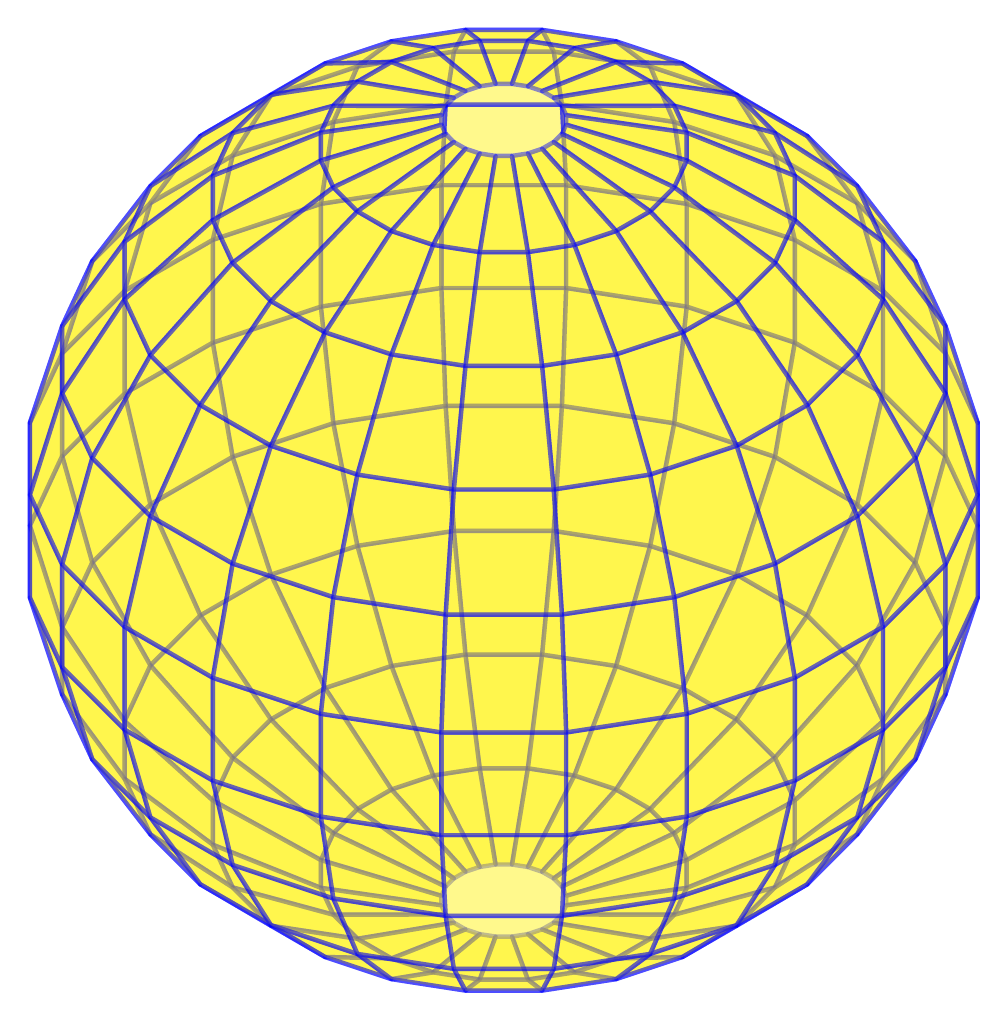
\begin{tikzpicture} [scale=5,isometricXYZ,ultra thick,opacity=.45,line join=round]
\def\h{7.5}
\foreach \t in {-135,-120,...,35}
  \foreach \f in {165,150,...,5}
    \draw [blue,fill=yellow]
          ({sin (\f-\h)*cos(\t-\h)},{sin(\f-\h)*sin(\t-\h)},{cos(\f-\h)})
       -- ({sin(\f-\h)*cos(\t+\h)},{sin(\f-\h)*sin(\t+\h)},{cos(\f-\h)})
       -- ({sin(\f+\h)*cos(\t+\h)},{sin(\f+\h)*sin(\t+\h)},{cos(\f+\h)})
       -- ({sin(\f+\h)*cos(\t-\h)},{sin(\f+\h)*sin(\t-\h)},{cos(\f+\h)})
       -- cycle;
\foreach \t in {210,195,...,40}
  \foreach \f in {165,150,...,5}
    \draw [blue,fill=yellow]
          ({sin (\f-\h)*cos(\t-\h)},{sin(\f-\h)*sin(\t-\h)},{cos(\f-\h)})
       -- ({sin(\f-\h)*cos(\t+\h)},{sin(\f-\h)*sin(\t+\h)},{cos(\f-\h)})
       -- ({sin(\f+\h)*cos(\t+\h)},{sin(\f+\h)*sin(\t+\h)},{cos(\f+\h)})
       -- ({sin(\f+\h)*cos(\t-\h)},{sin(\f+\h)*sin(\t-\h)},{cos(\f+\h)})
       -- cycle;
\end{tikzpicture}

%: sphere two
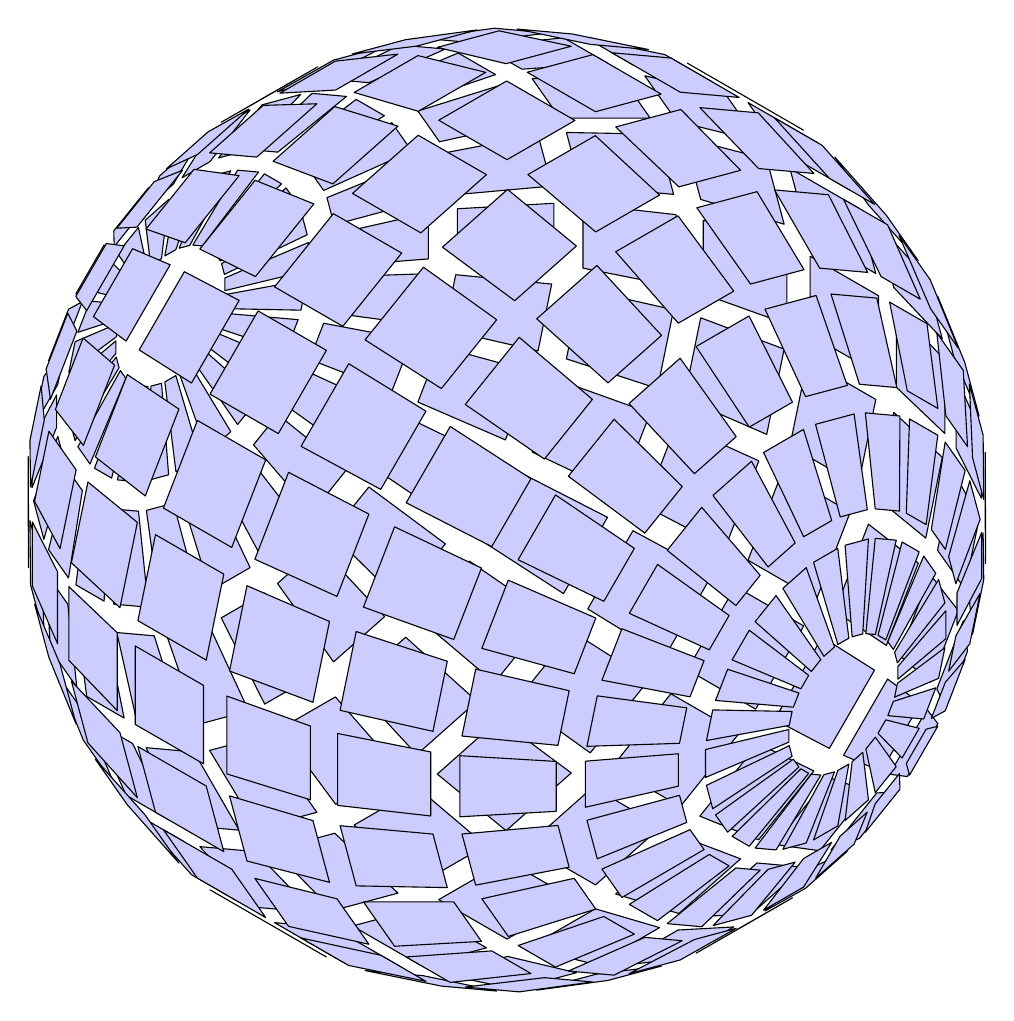
\begin{tikzpicture} [scale=5,isometricYZX,line join=round]
\def\h{5.75}
\foreach \t in {-135,-120,...,35}
  \foreach \f in {165,150,...,5}
    \draw [fill=blue!20]
          ({sin (\f-\h)*cos(\t-\h)},{sin(\f-\h)*sin(\t-\h)},{cos(\f-\h)})
       -- ({sin(\f-\h)*cos(\t+\h)},{sin(\f-\h)*sin(\t+\h)},{cos(\f-\h)})
       -- ({sin(\f+\h)*cos(\t+\h)},{sin(\f+\h)*sin(\t+\h)},{cos(\f+\h)})
       -- ({sin(\f+\h)*cos(\t-\h)},{sin(\f+\h)*sin(\t-\h)},{cos(\f+\h)})
       -- cycle;
\foreach \t in {210,195,...,40}
  \foreach \f in {165,150,...,5}
    \draw [fill=blue!20]
          ({sin (\f-\h)*cos(\t-\h)},{sin(\f-\h)*sin(\t-\h)},{cos(\f-\h)})
       -- ({sin(\f-\h)*cos(\t+\h)},{sin(\f-\h)*sin(\t+\h)},{cos(\f-\h)})
       -- ({sin(\f+\h)*cos(\t+\h)},{sin(\f+\h)*sin(\t+\h)},{cos(\f+\h)})
       -- ({sin(\f+\h)*cos(\t-\h)},{sin(\f+\h)*sin(\t-\h)},{cos(\f+\h)})
       -- cycle;
\end{tikzpicture}

%: sphere three
\begin{center}
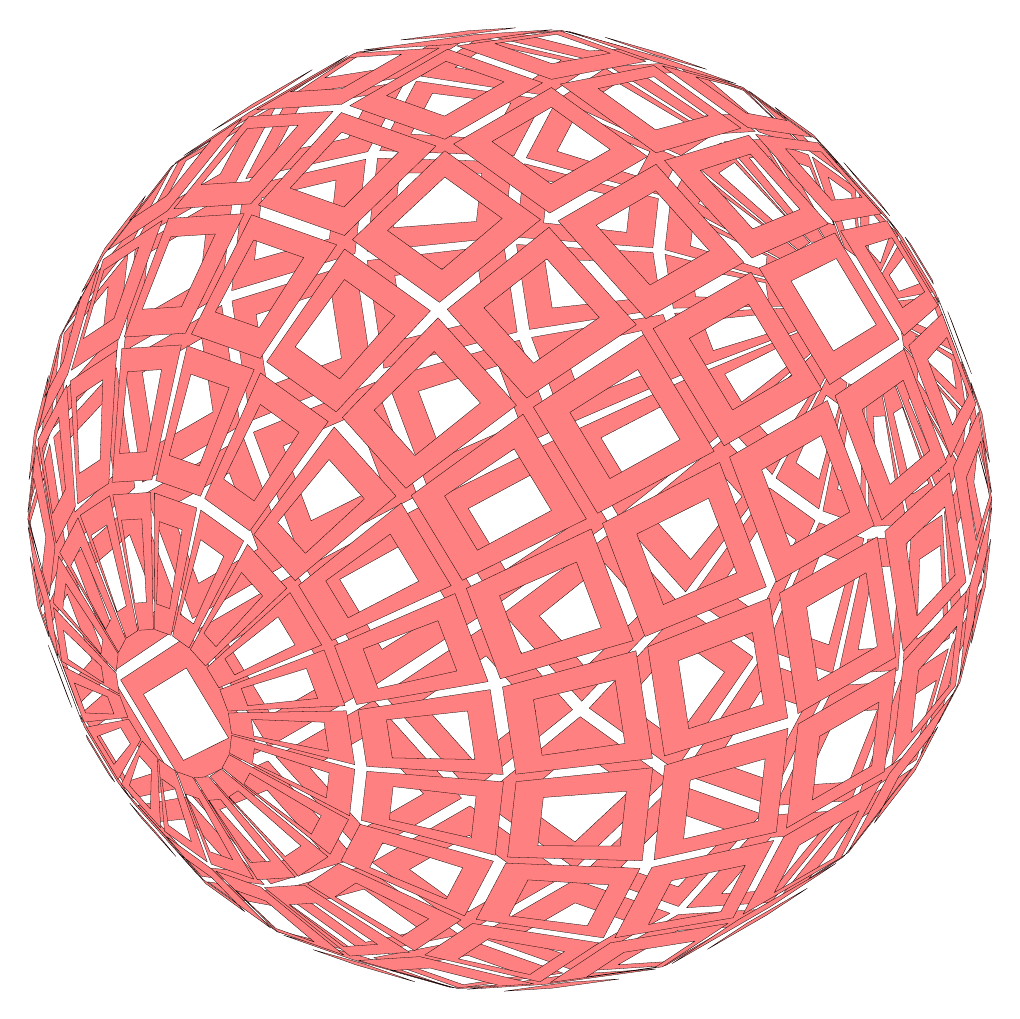
\begin{tikzpicture} [scale=5,isometricZXY,ultra thin,even odd rule,line join=round]
\def\h{8.25}
\def\k{5}
\foreach \t in {-133,-115,...,33}
  \foreach \f in {162,144,...,18}
    \draw [fill=red!50]
          ({sin (\f-\h)*cos(\t-\h)},{sin(\f-\h)*sin(\t-\h)},{cos(\f-\h)})
       -- ({sin(\f-\h)*cos(\t+\h)},{sin(\f-\h)*sin(\t+\h)},{cos(\f-\h)})
       -- ({sin(\f+\h)*cos(\t+\h)},{sin(\f+\h)*sin(\t+\h)},{cos(\f+\h)})
       -- ({sin(\f+\h)*cos(\t-\h)},{sin(\f+\h)*sin(\t-\h)},{cos(\f+\h)})
       -- cycle
          ({sin (\f-\k)*cos(\t-\k)},{sin(\f-\k)*sin(\t-\k)},{cos(\f-\k)})
       -- ({sin(\f-\k)*cos(\t+\k)},{sin(\f-\k)*sin(\t+\k)},{cos(\f-\k)})
       -- ({sin(\f+\k)*cos(\t+\k)},{sin(\f+\k)*sin(\t+\k)},{cos(\f+\k)})
       -- ({sin(\f+\k)*cos(\t-\k)},{sin(\f+\k)*sin(\t-\k)},{cos(\f+\k)})
       -- cycle;
\foreach \t in {209,191,...,33}
  \foreach \f in {162,144,...,18}
    \draw [fill=red!50]
          ({sin (\f-\h)*cos(\t-\h)},{sin(\f-\h)*sin(\t-\h)},{cos(\f-\h)})
       -- ({sin(\f-\h)*cos(\t+\h)},{sin(\f-\h)*sin(\t+\h)},{cos(\f-\h)})
       -- ({sin(\f+\h)*cos(\t+\h)},{sin(\f+\h)*sin(\t+\h)},{cos(\f+\h)})
       -- ({sin(\f+\h)*cos(\t-\h)},{sin(\f+\h)*sin(\t-\h)},{cos(\f+\h)})
       -- cycle
          ({sin (\f-\k)*cos(\t-\k)},{sin(\f-\k)*sin(\t-\k)},{cos(\f-\k)})
       -- ({sin(\f-\k)*cos(\t+\k)},{sin(\f-\k)*sin(\t+\k)},{cos(\f-\k)})
       -- ({sin(\f+\k)*cos(\t+\k)},{sin(\f+\k)*sin(\t+\k)},{cos(\f+\k)})
       -- ({sin(\f+\k)*cos(\t-\k)},{sin(\f+\k)*sin(\t-\k)},{cos(\f+\k)})
       -- cycle;
\end{tikzpicture}
\end{center}

\end{document}
